\documentclass[12pt]{article}

\usepackage{float}
\usepackage{amsmath}
\usepackage{amsfonts}
\usepackage{graphicx}
\graphicspath{ {./images/} }

\usepackage{listingsutf8}
\usepackage[utf8]{inputenc}

\usepackage[a4paper, total={16cm, 23.7cm}]{geometry}
\DeclareMathSizes{12}{13}{10}{8}
\setlength\parindent{0pt}

\usepackage[colorlinks=true,urlcolor=blue]{hyperref}
\usepackage{color}

\newcommand*\diff{\mathop{}\!\mathrm{d}}
\newcommand*\Diff[1]{\mathop{}\!\mathrm{d^#1}}
\newcommand\tab[1][.7cm]{\hspace*{#1}}
\renewcommand{\refname}{}

\fontfamily{phv}

% !TeX spellcheck = en_US


\begin{document}	
	
	%----------------------------------------------------------------------------
	% TITLE
	%----------------------------------------------------------------------------
	\begin{center}
		\Huge Performance optimization of CERN's LHCb online data processing software \\
		\Large Thesis report\\
		\vspace{1pc}
		\huge Péter Kardos \\
		\large 2018-2019
	\end{center}
	
	
	%----------------------------------------------------------------------------
	% === ABSTRACT ===
	%----------------------------------------------------------------------------
	\section{Abstract}
	
	\color{red}
	write at the end \\
	100-200 words \\
	- what's the problem \\
	- how was it solved \\
	- what are the results \\
	- conclusion: what it means for the future \\
	must be understandable without extra info	
	\color{black}
	\vspace{1.5pc}
		
	PLACEHOLDER
	So this abstract should be about 100-200 words so I'm just writing some natural text to act as a placeholder. By looping this text a few times, I can probably make a 150 word section. So this abstract should be about 100-200 words so I'm just writing some natural text to act as a placeholder. By looping this text a few times, I can probably make a 150 word section. So this abstract should be about 100-200 words so I'm just writing some natural text to act as a placeholder. By looping this text a few times, I can probably make a 150 word section. So this abstract should be about 100-200 words so I'm just writing some natural text to act as a placeholder. By looping this text a few times, I can probably make a 150 word section. So this abstract should be about 100-200 words so I'm just writing some natural text to act as a placeholder. By looping this text a few times, I can probably make a 150 word section.
	
	
	%----------------------------------------------------------------------------
	% === Introduction ===
	%----------------------------------------------------------------------------
	\newpage
	\section{Introduction}
	
	\color{red}
	describe the problem in detail \\
	specific to my thesis: \\
	environment: \\
	- CERN's goals/activity \\
	- CERN's hardware infrastructure (accelerators, experiments) \\
	- LHCb's hardware infrastructure \\
	- LHCb's software reconstruction system \\
	problem: \\
	- event rate from detector \\
	- slow trigger $\rightarrow$ loss of physics (ACTUAL PROBLEM) \\
	- by optimizing individual algorithms (in this thesis) \\
	\color{black}
	\vspace{1.5pc}
	
	CERN (European Organization for Nuclear Research) is an international high energy experimental physics research organization situated near Geneva, on the Franco-Swiss border. CERN is host to the world's largest particle accelerator and numerous experiments which aim to provide a better understanding of the universe. The goals of the experiments, among others, are to verify the standard model of particles \textcolor{cyan}{TODO: list some more goals}.
	\cite{cern_about}
	
	
	\subsection{The accelerator complex \cite{cern_accel_complex}}
	
	\begin{figure}[H]
		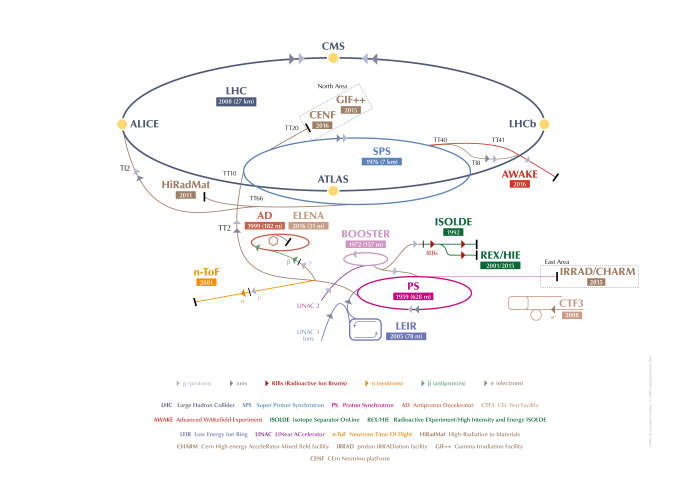
\includegraphics[width=\textwidth]{accelerator_complex}
		\label{fig_accel_complex}
		\caption{Schematic view of CERN's particle accelerators. Our main concern, LHC, is the largest circle shown on the top, along with the four main experiments, CMS, ALICE, ATLAS and LHCb, marked with a yellow dot.}
	\end{figure}
	
	LHC (Large Hadron Collider) is CERN's largest particle accelerator, or particle collider to be more precise. LHC is primarily used to accelerate protons. The particles are accelerated in multiple stages, in other words, a smaller accelerator accelerates them as much as it can, then particles are transferred to a larger accelerator which bumps them to an even higher energy, finally ending up in LHC at 7 TeV \cite{lhc_energy}.
	
	In the LHC, there are two proton beams circling at the same time, but in opposite directions. These beams are made to cross each-other at certain points, giving way to proton-proton collisions at 13-14 TeV. The collision produce a large number of various particles, which then fly away from the collision point.
	
	
	\subsection{Experiments on LHC}
	
	The four largest experiments, ATLAS, CMS, ALICE and LHCb, have their dedicated underground rooms at the collisions points. In these rooms, huge detectors are installed which are meant to track the particles created during the the collision. ATLAS and CMS have general purpose detectors aimed to examine a wide range of physics phenomena, while ALICE and LHCb have specialized detectors. The raw data produced by detectors is processed by software to identify each particle and their paths, and finally physicists analyze the results.
	
	
	\subsection{LHCb detector hardware}
	
	To understand how particle paths are reconstructed in software, one must understand the various parts of the detector used for tracking.
	
	\begin{figure}[H]
		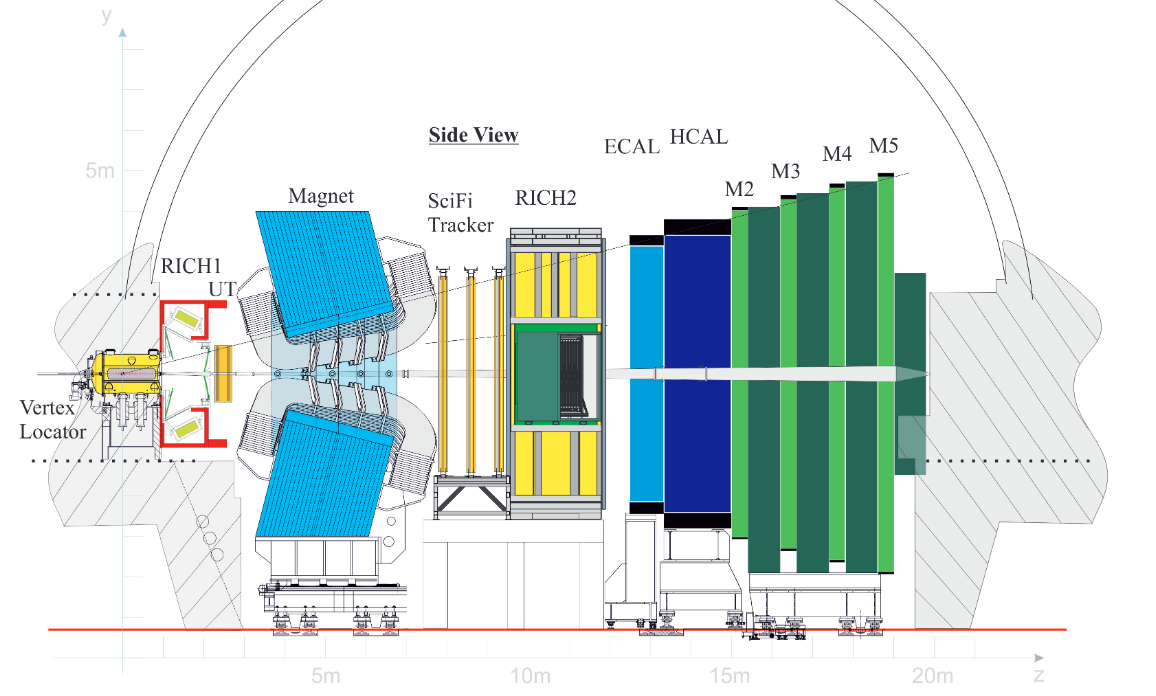
\includegraphics[width=\textwidth]{lhcb_geometry_upgrade}
		\label{fig_lhcb_geometry}
		\caption{Side view of the LHCb detector.}
	\end{figure}

	Figure \ref{fig_lhcb_geometry} depicts the LHCb detector from the side, making detector layers visible. The beam 
	
	\subsection{LHCb software reconstruction and computing hardware}
	
	%----------------------------------------------------------------------------
	% === TBD ===
	%----------------------------------------------------------------------------
	\section{Choosing optimization targets}
	
	\color{red}
	Explain the choice of initial choice of algorithms, based on the pie chart diagram and logical reasoning of our goals (i.e. what's needed).	
	\color{black}
	
	%----------------------------------------------------------------------------
	% === TBD ===
	%----------------------------------------------------------------------------
	\section{Parametrized Kalman Fitter}
	
	\subsection{What is fitting}
	
	%----------------------------------------------------------------------------
	% === TBD ===
	%----------------------------------------------------------------------------
	\section{TBD}
	
	%----------------------------------------------------------------------------
	% === Conclusion ===
	%----------------------------------------------------------------------------
	\section{Conclusion}
	
	\color{red}
	- summarize my own contributions \\
	- summarize achieved results \\
	- make conclusions about them \\
	- how it affects the future \\
	BRIEFLY
	\color{black}

	
	%----------------------------------------------------------------------------
	% REFERENCES
	%----------------------------------------------------------------------------
	\section{References}
	
	\begin{thebibliography}{asd}
		\bibitem{cern_about} About CERN: \\
			\url{https://home.cern/about}
		\bibitem{cern_accel_complex} The accelerator complex: \\
			\url{https://home.cern/about/accelerators}
		\bibitem{lhc_desc} About the Large Hadron Collider: \\
			\url{https://home.cern/topics/large-hadron-collider}
		\bibitem{lchb_desc} About the Large Hadron Collider beauty experiment: \\
			\url{https://home.cern/about/experiments/lhcb}
		\bibitem{lhc_energy} Energy of the LHC: \\
			\url{https://home.cern/about/engineering/restarting-lhc-why-13-tev}
	\end{thebibliography}

\end{document}





















